\newcommand*{\DesignPattern}{\begingroup

%----------------------------------------------------------------------------------------
%	Design Pattern
%----------------------------------------------------------------------------------------
\chapter{Design Pattern}\label{ch:designPatterns}
One benefit of C++ as an OOP language, which was not mentioned yet, is the suitability of using design patterns within the development process. 
The book 'Design Patterns: Elements of Reusable Object-Oriented Software' is a basic catalog of useful design patterns and was published by the authors Erich Gamma, Richard Helm, Ralph Johnson and John Vlissides. The authors are often just known as Gang of Four (GoF). According to GoF every design pattern describes a problem and the core of the solution for the problem in a way where the solution can be reused million times without redundancy. \cite[cf.][27 - 28]{GoF2015} A design pattern contains four characteristics:

\begin{itemize}
\item A significant name which refers to problem, solution as well as the effect of the design patterns.
\item The problem in which the use of the design pattern might be helpful. This problem defines specific constraints and requirements for architecture, behavior and algorithms.
\item The solution for the problem describes an abstract definition of the architectural design for solving the problem.
\item The consequences and effects of the usage of the design pattern. This includes advantages and disatvantages in many aspects like memory usage, timing, flexibility, portability, extensibility or reusability. Some of them are measurable and comparable, others are only visible within the work of the software architect.
\end{itemize}

\noindent Usually the use of design patterns effect a combination of advantages and disatvantages, so the software architect must decide whether the use is reasonable or not. As the name suggests, a design pattern is only a pattern. The solution does not describe or suggest a concrete implementation. No special facilities of particular programming languages are involved in the solution of the problem, which allows the use of design patterns for nearly every imperative programming language. In fact, unlike the first assumption of this chapter that the suitability of using design patterns would be a benefit of OOP languages, desing patterns are also available for the use with procedural programming languages like C. The book 'Design Patterns for Embedded Systems in C', written by Bruce Powel Douglass, offers a deep insight of the use of design patterns for the programming language C. Nevertheless the beneficial connection between OOP languages and design patterns is ubiquitous. Not least because most of the design patterns presented by GoF assume an architectural design with objects. \cite[cf.][29]{GoF2015} GoF classifies design patterns in its purpose and its scope. The purpose can be categorized in:

\begin{itemize}
  \item Creational patterns: with focus on the creation of new objects.
  \item Structural patterns: define the composition of classes and objects.
  \item Behavioral patterns: characterize the way of interaction between classes and objects.
\end{itemize}

\noindent In addition, the scope of a design pattern can be categorized in:

\begin{itemize}
  \item Class based patterns: influence the relation between classes, which is static and already determined at compile time.
  \item Object based patterns: influence the relation between objects at runtime.
\end{itemize}

\noindent Within the survey, mentioned in section \ref{sec:modernCplusplus}, the 30 participants were asked to name up to three of their most frequently used design patterns. The result shows a wide variety of design patterns with the singleton pattern as favourite. (Figure \ref{fig:frequentlyUsedDesignPatterns})

\begin{figure}[h]{}
\centering
\mbox{\frame{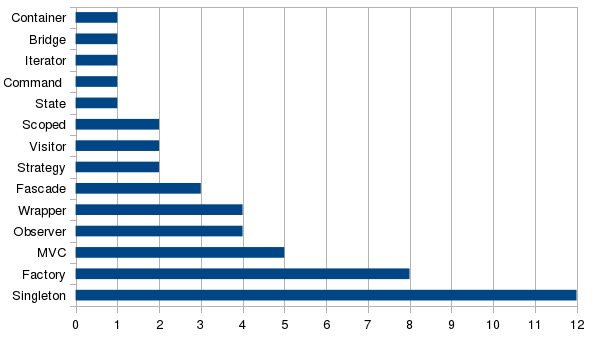
\includegraphics[width=\textwidth]{Images/FrequentlyUsedDesignPattern.png}}}
\caption{Frequently used design patterns}
\label{fig:frequentlyUsedDesignPatterns}
\end{figure}

\FloatBarrier

%----------------------------------------------------------------------------------------
%	Design Patterns on Embedded Systems
%----------------------------------------------------------------------------------------
\section{Design Patterns on Embedded Systems}\label{sec:designPatternOnEmbeddedSystems}
\noindent Design patterns can improve the software architecture of embedded systems in many ways. As mentioned in chapter \ref{ch:embeddedReactiveSystems} an embedded system interacts with its environment. In many cases the behavior of the system depends on information received from the environment or other systems. During the development process the designer does only know what kind of messages could come in. Arrival time, occurrences and the order of the messages are unknown. The use of design patterns like the factory method pattern or the strategy pattern provide a more dynamic behavior of the system. Constraints in time or availability of memory require efficient software which can be reached with design patterns like the flyweight pattern. For many more problems and challenges within the design process of an embedded system appropriate design patterns are available.

%----------------------------------------------------------------------------------------
%	Implementation in C++11
%----------------------------------------------------------------------------------------
\section{Implementation in C++11}\label{sec:designPatternImplementation}
\noindent Literatur and the internet offer many examples of how to implement concrete design patterns in C++. Few of these examples use C++11 facilities. For example the actual release of GoF from 2015 also includes concrete implementations in C++ and non of them include the facilities released with C++11. A reason for this rarely representation within concrete examples is hard to find. The following selected design patterns shall give an deeper understanding of how does C++11 have an impact on the implementation of design patterns in C++ for finding an answer for the question whether C++11 is beneficial or not.

%So why is C++11 still rarely represented within concrete examples of implementation? The following selected design patterns shall give an deeper understanding of how does C++11 have an impact on the implementation of design patterns in C++.

\endgroup}
